% !TeX root = ../main.tex
% =====================================================================
% Chapter 4 -- Approach  (restructured)
%
% Preamble requirements:
%   \usepackage{amsmath,amssymb,booktabs}
%   \usepackage{hyperref}
%   \usepackage{cleveref}          % load LAST
%
%   \newcounter{assumption}
%   \renewcommand{\theassumption}{A\arabic{assumption}}
%   \crefname{assumption}{Assumption}{Assumptions}
%   \Crefname{assumption}{Assumption}{Assumptions}
%   \newcommand{\assum}[2]{\refstepcounter{assumption}\item[\theassumption\ #2]\label{#1}}
%
%   \newcounter{requirement}
%   \renewcommand{\therequirement}{R\arabic{requirement}}
%   \crefname{requirement}{Requirement}{Requirements}
%   \Crefname{requirement}{Requirement}{Requirements}
%   \newcommand{\req}[2]{\refstepcounter{requirement}\item[\therequirement\ #2]\label{#1}}
% =====================================================================

\chapter{Approach}\label{chap:approach}

This chapter develops the design of a breathable distributed real-time system.
It begins with the system vision and the conditions that trigger reconfiguration
(Sections~\ref{sec:breathability} and~\ref{section:approachusecases}), formalises
the workload, the platform and the notion of a migration event
(Section~\ref{sec:systemmodel}), states the assumptions under which the design
is developed (Section~\ref{sec:assumptions}) and the requirements it must
satisfy (Section~\ref{sec:requirements}), and derives from these the
architecture (Section~\ref{sec:architecture}) and the criticality-stratified
migration design (Section~\ref{sec:strategyoverview}) that the following
chapters realise. The design decisions taken along the way, and the
alternatives rejected, are collected in Section~\ref{sec:designdecisions}. The
chapter closes by delimiting the safety claims made in this work
(Section~\ref{sec:safetyscope}) and by relating each mechanism to the chapter
in which it is described (Section~\ref{sec:designstatus}).

Parts of the architecture and of the system model presented here were published
in~\parencite{delgadillo_rage26}.
% TODO: confirm the exact self-citation wording required by the examination
% regulations, and add the corresponding statement to the front matter.

% =====================================================================
\section{Breathability}\label{sec:breathability}

Conventional distributed real-time systems fix the assignment of tasks to
computing nodes at design time. The assignment is then the subject of an
offline schedulability analysis, and the guarantees derived from that analysis
hold for as long as the assumptions underlying it hold: the task set does not
change, and the set of functioning nodes does not change. Neither condition is
satisfied in a modern vehicle, where computing resources appear and disappear
as devices fail, restart for updates, are powered down for energy reasons, or
as edge infrastructure enters and leaves communication range.

This dissertation therefore develops a system that is \emph{breathable}. A
distributed real-time system is called breathable if the assignment of tasks to
nodes is revisable at runtime, and if every revision preserves the timing
guarantees of tasks in order of their criticality: guarantees given to tasks of
higher criticality are never relaxed in favour of tasks of lower criticality.
The metaphor is deliberate --- the system expands onto additional resources
when they become available and contracts onto the remaining ones when they do
not, shedding load from the least critical end of the task set rather than
failing as a whole.

Breathability is triggered by two categories of condition:

\begin{enumerate}
  \item \emph{Changes to the task set.} Tasks are added to or removed from the
    global task queue, or the load they impose changes. An increase may exceed
    the capacity of the current assignment; a decrease may permit consolidation
    onto fewer nodes and the powering down of the remainder.

  \item \emph{Changes to the resource set.} Physical devices are added or
    removed, whether through hardware failure, restart after an update, or
    deliberate power management. Virtual devices hosted on Mobile Edge
    Computing~(MEC) infrastructure become reachable or unreachable as a function
    of vehicle position, and the latency of the link to them varies.
\end{enumerate}

Reacting to either category requires the same underlying capability: moving a
running task from the node currently executing it to another node, without
losing the progress it has made and without violating the timing guarantees of
that task or of any other. Providing that capability, and establishing the
conditions under which it preserves timing guarantees, is the subject of this
dissertation. The decision of \emph{which} tasks to move and \emph{where} is a
separate problem, addressed in prior work of this research
group~\parencite{delgadillo_jlpea22} and treated here as an external component
(\cref{asm:planner}).

% =====================================================================
\section{Use Cases}\label{section:approachusecases}

The following four scenarios make the triggering conditions concrete. They are
referred to throughout the dissertation and form the basis of the evaluation
scenarios in Chapter~\ref{chap:evaluation}.

\paragraph{UC1 --- Physical device failure.}
A physical ECU becomes unavailable. Tasks of high criticality that were
executing on it must resume elsewhere with minimal and, above all, bounded
downtime; the design provides for this by maintaining a prepared backup node
for such tasks. Tasks of low criticality, both those displaced from the failed
device and those already resident on the node that absorbs the load, are
redistributed across the remaining hardware. Where the remaining hardware
cannot accommodate the entire task set, tasks of high criticality are served
first and tasks of low criticality skip jobs, or are deferred entirely, until
load decreases or capacity is restored. This use case exercises
\cref{req:transfer,req:criticality,req:timing}.

\paragraph{UC2 --- Change in task load.}
The load imposed by the task set rises or falls. A rise may require
redistribution across nodes, or the activation of a node previously held in
standby, in order to reach a configuration in which every task is schedulable.
A fall permits the converse: consolidation onto fewer nodes and the powering
down of the remainder for energy efficiency. In both directions, the migration
of highly critical tasks is avoided except where no alternative exists, since
each migration introduces an additional opportunity for failure; this
preference is expressed as a penalty in the planning component
(\cref{asm:planner}) rather than as a prohibition. This use case exercises
\cref{req:criticality,req:footprint}.

\paragraph{UC3 --- Capability-driven offload to the MEC.}
MEC infrastructure becomes available and hosts resources a task can exploit ---
greater computational capacity, or sensor data from beyond the vehicle. A task
able to benefit is migrated to a virtual node. Because the availability of the
infrastructure is a function of vehicle position, such a task retains a
counterpart on physical hardware that provides basic functionality, while the
migrated instance provides enhanced functionality for as long as the
infrastructure remains reachable. A path-planning function illustrates the
pattern: the local counterpart follows the current route safely, while the
offloaded instance computes alternative routes using traffic and incident data
available only at the edge. This use case exercises
\cref{req:portability,req:timing}.

\paragraph{UC4 --- Load-driven offload to the MEC.}
MEC infrastructure is available and the load on the physical devices is
critically high, for instance following the device failure of UC1. Tasks of low
criticality that would otherwise be starved are offloaded to virtual nodes for
as long as the infrastructure remains reachable, accepting the additional
latency of the external link in exchange for continued service. An infotainment
streaming service is a representative example. The results such tasks produce
must be forwarded back into the vehicle network, which requires a
task-independent forwarding mechanism on the vehicle side. This use case
exercises \cref{req:transfer,req:criticality}.

\bigskip
\noindent
UC1 and UC2 are driven by changes within the vehicle and are served by
migration between physical nodes. UC3 and UC4 both involve virtual nodes but
differ in what motivates the migration --- capability in UC3, capacity in UC4
--- and therefore in what happens when the link is lost: in UC3 the local
counterpart continues unaffected, whereas in UC4 the offloaded task must be
recalled or dropped. This distinction is developed in
Section~\ref{sec:strategyoverview}.


% =====================================================================
\section{System Model}\label{sec:systemmodel}

This section introduces the notation used throughout the remainder of this
dissertation. The model is deliberately compact: it captures only those
properties of tasks, nodes and migration events that are needed to state the
design requirements of Section~\ref{sec:requirements}, to formulate the
migration cost model of Chapter~\ref{chap:migration}, and to interpret the
measurements of Chapter~\ref{chap:evaluation}. A summary of the symbols is
given in Table~\ref{tab:notation}.

\subsection{Nodes and Sub-Nodes}\label{subsec:nodemodel}

The system follows a master--worker model. A single \emph{master node}
coordinates a set of \emph{worker nodes} that execute the task set. Where the
distinction is not at issue, worker nodes are referred to simply as nodes.

A \emph{node} is a device: a physical Electronic Control Unit~(ECU) within the
vehicle, or a virtual ECU hosted on Mobile Edge Computing~(MEC) infrastructure
outside it. A node comprises one or more \emph{sub-nodes}, a sub-node being an
independently scheduled instance of the execution platform, owning a
scheduler and a task set of its own. A single-core node has one sub-node. A
multi-core node operated in Asymmetric Multiprocessing~(AMP) mode has one
sub-node per core, of which one is designated the \emph{master core} and acts
as the node's single point of contact towards the master node; the remainder
are \emph{slave cores}.

The distinction matters because the properties relevant to the design divide
between the two levels. Communication properties are properties of a device:
every core of an ECU reaches the master node over the same link and shares the
same hardware clock. Scheduling properties are properties of a core: each
runs its own scheduler and, under the reserved-core realisation of
Section~\ref{subsec:os:schedvariants}, may carry a criticality ceiling
different from that of its neighbours. Tasks are assigned to sub-nodes, not to
nodes.

The set of nodes is denoted $\mathcal{N} = \{\nu_1, \dots, \nu_m\}$, with
%
\begin{equation}\label{eq:nodemodel}
  \nu_j = \bigl(\,\theta_j,\; \Sigma_j,\; \beta_j,\; \delta_j,\;
                  \Delta_j,\; \Pi_j \,\bigr),
\end{equation}
%
where $\theta_j \in \{\textsf{physical}, \textsf{virtual}\}$ is the node type,
$\Sigma_j$ the set of system services the node can provide (network access,
specific sensors, peripherals), $\beta_j$ the bandwidth of the link to the
master node, $\delta_j$ the bounded latency of that link, $\Delta_j$ the bound
on the deviation of the node's clock from the global reference, and $\Pi_j$
its set of sub-nodes.

Each sub-node $\pi_k \in \Pi_j$ is characterised by
%
\begin{equation}\label{eq:subnodemodel}
  \pi_k = \bigl(\,f_k,\; \mu_k,\; L_k^{\max}\,\bigr),
\end{equation}
%
with $f_k$ the processor frequency, $\mu_k$ the memory available to guest
tasks, and $L_k^{\max}$ the \emph{criticality ceiling} introduced in
Section~\ref{subsec:criticalitymodel}. Where a property of the node
containing a sub-node is required, it is written with the node's index; thus
$\delta_j$ is the link latency applicable to every $\pi_k \in \Pi_j$.

Nodes of type \textsf{virtual} are hosted on MEC infrastructure. Their
defining property in this model is not their virtualisation technology but the
fact that $\delta_j$ is neither controlled by the vehicle nor bounded by an
in-vehicle network, which is the formal reason for the criticality ceiling
carried by their sub-nodes.

All nodes share a common instruction set architecture, ARM~AArch64 in the
realisation described in Chapter~\ref{chap:os}. Heterogeneity is therefore
supported at the level of the software stack, the hardware peripherals and the
processor frequency, but not at the level of the instruction
set~(\cref{asm:isa}).

\subsection{Tasks, Jobs and Criticality}\label{subsec:taskmodel}

The workload is a set of independent tasks $\Gamma = \{\tau_1, \dots,
\tau_p\}$ held in a global task queue by the master node. Each task is
characterised by the tuple
%
\begin{equation}\label{eq:taskmodel}
	\tau_i = \bigl(\,\chi_i,\; \mathbf{C}_i,\; T_i,\; D_i,\; N_i,\; r_i,\;
	S_i,\; E_i,\; \Sigma_i \,\bigr),
\end{equation}
%
with the following components:

\begin{itemize}
	\item $\chi_i \in \mathcal{L}$ --- the \emph{criticality level} of the
	task, drawn from the ordered set $\mathcal{L}$ defined in
	Section~\ref{subsec:criticalitymodel}.
	
	\item $\mathbf{C}_i = \bigl(C_i(\ell)\bigr)_{\ell \in \mathcal{L}}$ --- the
	vector of worst-case execution time~(WCET) estimates, one per criticality
	level, following the mixed-criticality task model of
	Vestal~\parencite{vestal2007}. The estimates are monotonically
	non-decreasing in the criticality level, $\ell_1 \leq \ell_2 \Rightarrow
	C_i(\ell_1) \leq C_i(\ell_2)$, reflecting the increasing pessimism
	required by higher assurance levels. Execution times are
	platform-dependent and are specified relative to a reference processor
	frequency; the estimate applicable on sub-node $\pi_k$ is written
	$C_i^{k}(\ell)$.
	
	\item $T_i$ --- the period, and $D_i \leq T_i$ the relative deadline
	(constrained-deadline model).
	
	\item $N_i \in \mathbb{N} \cup \{\infty\}$ --- the number of jobs the task
	is to execute, and $r_i$ its release time. This parameter unifies the
	treatment of periodic and sporadic workloads: a task with $N_i = \infty$
	is a conventional periodic task, a task with $N_i = 1$ models a
	single sporadic activation, and finite $N_i > 1$ models a bounded batch of
	activations, a form used for lower-criticality workloads that may be
	admitted or deferred in batches~(Assumption~\ref{asm:periodic}).
	
	\item $S_i$ --- the size of the task's \emph{checkpoint}, i.e.\ the
	serialised state that must be preserved across a migration event, and
	$E_i$ the size of its executable image. These two parameters do not
	appear in classical real-time task models. They are introduced here
	because, in a system where task-to-node binding is revised at runtime,
	the cost of that revision is dominated by the transfer of $S_i$ and
	$E_i$; they are consequently the inputs to the migration cost model of
	Section~\ref{sec:migrationcost}.
	
	\item $\Sigma_i$ --- the set of system services the task requires. A task
	may only be assigned to a sub-node of a node $\nu_j$ with
	$\Sigma_i \subseteq \Sigma_j$.
\end{itemize}

A \emph{job} $J_{i,q}$ is the $q$-th activation of task $\tau_i$. Jobs follow
the sense--think--act pattern common in cyber-physical systems: a job reads
its inputs, restores the task state produced by $J_{i,q-1}$, computes, emits
its outputs, and persists the state for $J_{i,q+1}$. The task state is the
only information that crosses the boundary between consecutive jobs; this
property is what makes the job boundary a natural quiescent point and is the
basis for Assumption~\ref{asm:jobboundary}.

\subsection{Criticality Levels and Node Ceilings}\label{subsec:criticalitymodel}

Criticality levels are drawn from a finite ordered set $\mathcal{L}$ modelled
on the Automotive Safety Integrity Levels~(ASIL) of
ISO~26262~\parencite{iso26262_2018}. Conceptually, $\mathcal{L}$ may contain
any number of levels; the design of the migration strategies in
Chapter~\ref{chap:migration} is formulated for arbitrary $|\mathcal{L}|$,
while the implementation and the evaluation use the two-level instantiation
$\mathcal{L} = \{\textsf{LO}, \textsf{HI}\}$ that is standard in the
mixed-criticality literature~\parencite{burns2017}. The rationale for this
restriction is that the design problems addressed here occur at the two ends
of the criticality spectrum --- bounded, resource-expensive migration at the
top, and flexible, resource-efficient migration at the bottom --- and that
intermediate levels are addressed by combining the two mechanisms rather than
by introducing a third one; this is discussed further in
Section~\ref{sec:intermediatelevels}.

Each sub-node carries a criticality ceiling $L_k^{\max}$: the highest
criticality level a task may have to be admissible on that sub-node. Ceilings are the
mechanism by which platform properties are translated into scheduling
constraints. In particular, virtual nodes are assigned a ceiling strictly
below the highest level, because the latency of the link to MEC
infrastructure is not bounded by any in-vehicle mechanism and because the
availability of the infrastructure itself is a function of vehicle position
rather than of system state. A task $\tau_i$ is admissible on sub-node
$\pi_k$ of node $\nu_j$ only if
%
\begin{equation}\label{eq:admissibility}
	\chi_i \leq L_k^{\max}
	\quad\wedge\quad
	\Sigma_i \subseteq \Sigma_j
	\quad\wedge\quad
	\text{the local schedulability test of $\pi_k$ admits $\tau_i$.}
\end{equation}

\subsection{Migration Events}\label{subsec:migrationmodel}

A \emph{migration event} is denoted
%
\begin{equation}
	\mathcal{M}\bigl(\tau_i,\, \pi_{\mathrm{src}},\, \pi_{\mathrm{dst}},\, t\bigr),
\end{equation}
%
the transfer of the execution of task $\tau_i$ from source sub-node
$\pi_{\mathrm{src}}$ to destination sub-node $\pi_{\mathrm{dst}}$, initiated
at time $t$. A migration event is \emph{admissible} if
Equation~\ref{eq:admissibility} holds for $\tau_i$ on $\pi_{\mathrm{dst}}$,
and it is \emph{timing-preserving} if no job of $\tau_i$, and no job of any
task resident on either sub-node, misses its deadline as a consequence of the
event. Establishing the conditions under which migration events are
timing-preserving is the object of research question~RQ1 and is treated
quantitatively in Section~\ref{sec:migrationcost}.

Migration events are triggered by the master node in response to two
categories of condition, as introduced in
Section~\ref{sec:breathability}: a change in the task set $\Gamma$, or a
change in the node set $\Pi$ or in the properties of its members. The
decision procedure that selects which migrations to perform is outside the
scope of this dissertation and is treated as an external
component~(Assumption~\ref{asm:planner}).

\subsection{Time}\label{subsec:timemodel}

Nodes maintain a common notion of time through the Precision Time
Protocol~(PTP). The clock of node $\nu_j$ deviates from the global reference
by an offset bounded by $\Delta_j$, and $\Delta^{\max} = \max_j \Delta_j$
denotes the system-wide bound. Because the sub-nodes of a node share its
hardware clock, the offset is a property of the node and applies uniformly to
all of its sub-nodes. Deadlines are specified globally and compensated
locally: a task with global relative deadline $D_i$ is scheduled on a sub-node
of $\nu_j$ against the adjusted deadline
%
\begin{equation}\label{eq:deadlinecompensation}
	D_i' = D_i - \Delta_j - \delta_j .
\end{equation}
%
Because both correction terms are properties of the node rather than of the
task, the adjustment is uniform across the task set of every sub-node of that
node and therefore preserves the relative ordering of deadlines under
EDF-based policies. It
does, however, reduce the available slack on every task resident on the node,
and thus has a schedulability cost; this cost is quantified in
Section~\ref{sec:ptpevaluation}.

\begin{table}[t]
	\centering
	\caption{Summary of notation.}
	\label{tab:notation}
	\begin{tabular}{@{}ll@{}}
		\toprule
		Symbol & Meaning \\
		\midrule
		$\mathcal{N}$, $\nu_j$    & set of nodes (devices); individual node \\
		$\Pi_j$, $\pi_k$          & sub-nodes of node $\nu_j$; individual sub-node \\
		$\theta_j$, $\Sigma_j$    & node type; services offered by the node \\
		$\beta_j$, $\delta_j$     & link bandwidth and bounded latency of node $\nu_j$ \\
		$f_k$, $\mu_k$            & processor frequency and guest memory of sub-node $\pi_k$ \\
		$L_k^{\max}$              & criticality ceiling of sub-node $\pi_k$ \\
		$\Sigma_i$                & services required by task $\tau_i$ \\
		$\Gamma$, $\tau_i$        & task set; individual task \\
		$\chi_i$, $\mathcal{L}$   & criticality of a task; ordered set of criticality levels \\
		$C_i(\ell)$, $C_i^k(\ell)$ & WCET at level $\ell$; WCET at level $\ell$ on sub-node $\pi_k$ \\
		$T_i$, $D_i$, $D_i'$      & period, global relative deadline, compensated deadline \\
		$N_i$, $r_i$, $J_{i,q}$   & job count, release time, $q$-th job of $\tau_i$ \\
		$S_i$, $E_i$              & checkpoint size, executable image size \\
		$\Delta_j$, $\Delta^{\max}$ & clock offset bound of node $\nu_j$; system-wide bound \\
		$\mathcal{M}(\cdot)$      & migration event \\
		$\Delta_{\mathrm{mig}}$   & total migration cost (Section~\ref{sec:migrationcost}) \\
		\bottomrule
	\end{tabular}
\end{table}

% =====================================================================\section{Assumptions and Scope}\label{sec:assumptions}

The model of Section~\ref{sec:systemmodel} rests on a number of assumptions.
They are stated explicitly here, together with the reason each is made and an
indication of whether it is a fundamental restriction of the approach or a
scoping decision that could be relaxed without invalidating the design.

\begin{description}
	
	\assum{asm:independence}{Task independence.}
	Tasks share no data and impose no precedence constraints on one another;
	consequently no mutual-exclusion protocol is required between them.
	\emph{Rationale:} resource-sharing protocols for mixed-criticality systems
	are an active research area in their own
	right~\parencite{burns2017}, and admitting shared resources would
	conflate the cost of migration with the cost of releasing and re-acquiring
	locks across nodes. Isolating the migration mechanism requires isolating
	the tasks.
	\emph{Status:} scoping decision. It is the strongest assumption made here
	and the most consequential for automotive realism, since sensor-fusion and
	perception pipelines are typically chains of dependent components. Relaxing
	it requires a distributed resource-sharing protocol and is identified as
	future work in Section~\ref{sec:futurework}.
	
	\assum{asm:periodic}{Periodic task model with bounded job count.}
	All tasks are treated as periodic with a job count $N_i$, as defined in
	Equation~\ref{eq:taskmodel}.
	\emph{Rationale:} it unifies periodic and sporadic workloads under a single
	scheduling and migration treatment without weakening the analysis, since
	a sporadic task with minimum inter-arrival time $T_i$ is schedulable
	whenever the corresponding periodic task is.
	\emph{Status:} scoping decision with no significant loss of generality.
	
	\assum{asm:jobboundary}{Migration at job boundaries.}
	A migration event transfers a task only between two of its jobs; a job in
	progress is never relocated mid-execution.
	\emph{Rationale:} the job boundary is the point at which the task's
	complete state is, by construction, contained in the user-defined
	checkpoint structure~(Section~\ref{subsec:taskmodel}). Relocating a job in
	progress would require capturing the program counter, stack and heap, which
	imposes both a substantially larger state transfer and kernel-level
	snapshot machinery incompatible with the memory footprint targeted here.
	\emph{Status:} fundamental to the approach. It has the direct consequence
	that the observable disruption of a migration is bounded by the task period
	rather than by the transfer time, and it is therefore the assumption that
	makes the timing analysis of Chapter~\ref{chap:migration} tractable. Its
	granularity limitation is partially mitigated by intra-job checkpoints
	(Section~\ref{sec:checkpointing}).
	
	\assum{asm:statecapture}{Completeness of the declared state.}
	The state structure declared by the application developer captures all
	information required to resume the task correctly on another node.
	\emph{Rationale:} the checkpoint mechanism is cooperative rather than
	transparent; correctness of migration is therefore a property of the guest
	task, not of the platform alone.
	\emph{Status:} fundamental, and a genuine burden placed on the application
	developer. Chapter~\ref{chap:os} describes the library support provided to
	reduce this burden; verification of state completeness is not addressed.
	
	\assum{asm:isa}{Common instruction set architecture.}
	All nodes share the ARM~AArch64 instruction set.
	\emph{Rationale:} a single position-independent binary per task can then be
	deployed to any node. The alternatives --- maintaining one compiled binary
	per target, or introducing an intermediate representation with
	just-in-time compilation --- either multiply the artefacts the
	master node must manage and transfer, or add a runtime engine whose
	execution time is difficult to bound.
	\emph{Status:} fundamental to the cross-platform loading mechanism.
	Heterogeneity in software stack, peripherals and clock frequency is
	supported; heterogeneity in instruction set is not.
	
	\assum{asm:planner}{Migration planning as an external component.}
	The procedure that decides which tasks should execute on which nodes is
	treated as a black box that emits admissible assignments.
	\emph{Rationale:} task-to-node partitioning has been addressed in prior
	work of this research group~\parencite{delgadillo_jlpea22, blieninger1},
	and the contribution of this dissertation lies in the execution of the
	resulting migrations rather than in the decision itself. The interface to
	this component, and the mixed-criticality extensions required of it, are
	described in Chapter~\ref{chap:integration}.
	\emph{Status:} scoping decision.
	
	\assum{asm:masternode}{Reliable master node.}
	The master node is assumed to be available and correct; it is not
	replicated.
	\emph{Rationale:} the centralised model removes the need for distributed
	consensus and permits the partitioning decision to run on a node with
	substantially greater computational resources than the ECUs.
	\emph{Status:} scoping decision, and an acknowledged single point of
	failure. A production deployment requires master node redundancy or
	distributed coordination; this is discussed in
	Section~\ref{sec:futurework}.
	
	\assum{asm:network}{Bounded in-vehicle communication latency.}
	Communication between the master node and physical nodes exhibits a
	latency bounded by $\delta_j$. No such bound is assumed for links to
	virtual nodes.
	\emph{Rationale:} the in-vehicle network in the evaluation setup is a
	switched Ethernet segment without deterministic guarantees, and $\delta_j$
	is therefore an empirical rather than an analytical bound. Obtaining an
	analytical bound requires Time-Sensitive Networking~(TSN), which the
	architecture accommodates but which is not part of the present
	realisation.
	\emph{Status:} scoping decision; it is the reason the timing results of
	Chapter~\ref{chap:evaluation} are stated relative to a measured
	$\delta_j$. The absence of the corresponding assumption for virtual nodes
	is deliberate and is what confines them to a criticality ceiling below
	the highest level.
	
	\assum{asm:security}{Trusted deployment channel.}
	Executable images and checkpoints received by a node are assumed
	authentic; no authentication, encryption or integrity verification beyond
	a transmission checksum is performed.
	\emph{Rationale:} the mechanisms required --- signed binaries, attested
	loading, encrypted transport --- are well understood in isolation but
	interact with the timing analysis in ways that would obscure the
	migration costs this work sets out to characterise.
	\emph{Status:} scoping decision. It is noted explicitly because dynamic
	loading of executable code received over a vehicle-to-infrastructure link
	is a significant attack surface, and any deployment of this architecture
	must address it.
	
	\assum{asm:certification}{Certification is out of scope.}
	The platform is designed to be compatible with the requirements that
	ISO~26262 imposes on the temporal behaviour of safety-related functions,
	but no certification argument is constructed and no component of the
	system is certified.
	\emph{Rationale and status:} discussed in detail in
	Section~\ref{sec:safetyscope}, which states precisely which properties
	are claimed and which are not.
	
\end{description}

% =====================================================================\section{Requirements}\label{sec:requirements}

The use cases of Section~\ref{section:approachusecases}, interpreted under the
model and assumptions above, yield the following requirements on the system.
They are referenced throughout the remainder of the dissertation.

\begin{description}
	\req{req:transfer}{Execution transfer.}
	It shall be possible to halt the execution of a task on one node and
	resume it on another, such that the task continues to produce results
	without manual intervention and without duplicate or omitted jobs.
	
	\req{req:state}{State preservation.}
	A migration event shall preserve the task state required for subsequent
	jobs to produce correct results. Progress accumulated over previous jobs
	shall not be lost.
	
	\req{req:criticality}{Criticality differentiation.}
	Both the decision to migrate and the mechanism by which migration is
	executed shall depend on the criticality of the task. Higher-criticality
	tasks shall be favoured whenever resources are contended, and shall never
	be delayed by the migration of lower-criticality tasks.
	
	\req{req:timing}{Timing preservation.}
	The timing behaviour of the system during and after a migration event
	shall remain analysable. For tasks at the highest criticality level the
	migration cost shall be bounded and the bound shall be established
	analytically; for lower levels a probabilistic characterisation is
	sufficient.
	
	\req{req:portability}{Platform portability.}
	A task shall be deployable, without recompilation, to any node satisfying
	Equation~\ref{eq:admissibility}, irrespective of that node's software
	stack or virtualisation status.
	
	\req{req:footprint}{Resource proportionality.}
	The runtime and memory overhead imposed by the migration infrastructure
	shall be compatible with ECU-class hardware, and the resources reserved
	for a given migration strategy shall be proportionate to the criticality
	of the tasks it serves.
\end{description}

Requirements~\ref{req:transfer} and~\ref{req:state} are common to any task
migration mechanism. Requirements~\ref{req:criticality} and~\ref{req:timing}
are what distinguish this work from the prior art surveyed in
Chapter~\ref{chap:relatedwork}, and jointly they imply that a single migration
mechanism is insufficient: a mechanism fast and predictable enough
for~\ref{req:timing} at the highest criticality level necessarily reserves
resources on nodes that are not executing the task, which
violates~\ref{req:footprint} if applied to the whole task set. The
criticality-stratified design of Section~\ref{sec:strategyoverview}, with
distinct strategies per criticality tier, follows directly from this tension.

% =====================================================================
% =====================================================================
\section{Architectural Overview}\label{sec:architecture}

The model of Section~\ref{sec:systemmodel} is realised by the architecture
shown in Figure~\ref{fig:mig_diag}. A reconfiguring situation triggers a
redistribution of the tasks held in the global task queue. The queue and the
current node set $\Pi$ are supplied to the partitioning component, which
computes a task-to-node mapping subject to
Equation~\ref{eq:admissibility}. Where the mapping assigns a task to a node
other than the one currently executing it, a migration event
$\mathcal{M}(\tau_i, \pi_{\mathrm{src}}, \pi_{\mathrm{dst}}, t)$ is issued and
executed by the mechanisms of Chapter~\ref{chap:migration}.

\begin{figure}
	\centering
	\makebox[\textwidth]{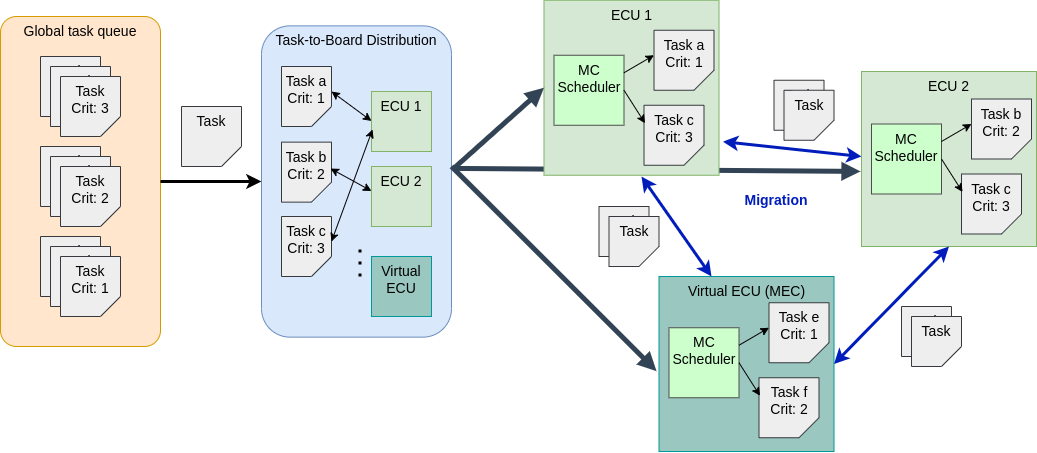
\includegraphics[width=\textwidth]{figures/Migration_Diag_new.png}}
	\caption{General system overview: the global task queue is partitioned onto
	         physical and virtual nodes, each running a mixed-criticality
	         scheduler, with migration events transferring tasks between them.}
	\label{fig:mig_diag}
\end{figure}

The architecture comprises four kinds of component.

The master node maintains the global task queue, tracks the set of
available nodes and their reported health, triggers the partitioning
component, and stores the artefacts required to start a task on any node: the
executable image, the most recent checkpoint, and the task's parameters
according to Equation~\ref{eq:taskmodel}. It is the single point of contact
for every node and, under \cref{asm:masternode}, is assumed reliable.
% TODO: state here that the current realisation hosts the master node on a
% workstation, and that nothing in the design prevents hosting it on an
% ECU-class device; forward-reference the evaluation setup.

The \emph{partitioning component} computes task-to-node mappings. It is
treated as a black box (\cref{asm:planner}); the interface it must satisfy,
and the extensions required of it to account for criticality and for migration
cost, are described in Chapter~\ref{chap:integration}.

\emph{Physical nodes} execute the majority of the task set. Each runs the
operating system described in Chapter~\ref{chap:os}, which provides a
mixed-criticality scheduler, dynamic task loading, and the checkpoint
mechanism. A physical ECU with several cores contributes one sub-node per core
under AMP, with the master core mediating between the master node and the
remaining cores. Nodes may be held in standby or powered down entirely to
conserve energy, and returned to service when UC1 or UC2 requires them.

\emph{Virtual nodes} are containerised instances of the same operating system
hosted on MEC infrastructure. They extend the capacity of the system and
provide access to services unavailable in the vehicle, but their sub-nodes
carry a criticality ceiling below the highest level for the reasons given in
Section~\ref{subsec:criticalitymodel}.

Two properties of this arrangement are worth stating explicitly. First, the
same task binary executes on physical and virtual nodes alike
(\cref{asm:isa}), so the master node stores one artefact per task rather than
one per task and platform. Second, because tasks are assigned to
sub-nodes rather than to nodes, migration between cores of one ECU and
migration between ECUs are the same operation at the level of the model,
differing only in the cost of the transfer --- a property the strategies of
Section~\ref{sec:strategyoverview} exploit.

% =====================================================================
\section{Criticality-Stratified Migration}\label{sec:strategyoverview}

\Cref{req:criticality,req:timing,req:footprint} cannot be satisfied by a single
migration mechanism. A mechanism that bounds migration cost tightly enough to
preserve the guarantees of the most critical tasks must avoid transferring the
executable image at migration time, which means the image must already be
resident on the destination --- and therefore on every node that is a candidate
destination. Applying that to the entire task set would reserve memory on every
node for every task, violating \cref{req:footprint} on ECU-class hardware.
Conversely, a mechanism that transfers the image on demand imposes a cost that
depends on $E_i$, on $S_i$, and on the state of the network, and is therefore
difficult to bound tightly.

The design resolves this by stratifying the mechanism by criticality. Three
strategies are defined; they are described in full in
Chapter~\ref{chap:migration} and summarised here only insofar as the
architecture depends on them.

\paragraph{The \textsf{HI} strategy} keeps a task resident in a standby state
on a subset of the nodes, with only one instance executing at any time and
runtime state held in a memory region shared between the candidate nodes and
accessible only to tasks of the corresponding criticality. Migration then
reduces to a stop signal on the source and a start signal on the destination,
with no transfer of the executable and no transfer of state. The cost is
correspondingly small and, more importantly, has small variance, which is what
makes it amenable to the analysis \cref{req:timing} demands at the highest
criticality level. The price is the memory reserved on every standby node and
the shared-memory infrastructure itself, which is why the strategy is confined
to the tasks that need it. For tasks requiring redundancy rather than
availability --- ASIL~D functions with a duplicated-execution requirement ---
the same arrangement supports executing several instances concurrently and
comparing their results.

\paragraph{The \textsf{LO} strategy} transfers the executable image and the
checkpoint over the network at migration time, allowing a task to be started on
any admissible node without prior reservation of resources there. The cost
depends on $E_i + S_i$ and on the network, and is characterised
probabilistically rather than by a tight bound. The strategy makes efficient
use of memory across the system and is applicable to the large majority of the
task set.

\paragraph{The virtual-node strategy} is a variant of the \textsf{LO} strategy
targeting nodes hosted on MEC infrastructure. It differs in that the
destination must first be instantiated --- the master node requests the
creation of a container --- and in that the link latency $\delta_j$ is neither
bounded nor under the control of the vehicle. Both differences are reasons the
criticality ceiling of virtual nodes lies below the highest level.

\medskip
\noindent
Intermediate criticality levels are addressed by combining these mechanisms
rather than by introducing further ones. Two combinations are available. A task
may be held in standby, as under the \textsf{HI} strategy, but coordinated over
the ordinary network rather than through shared memory, trading determinism for
a lower memory footprint. Alternatively, the standby set may be reduced: in a
system with two high-criticality sublevels, tasks at the upper sublevel are held
in standby on every node while those at the lower sublevel are held on only a
few, guaranteeing a prepared destination for the former while consuming fewer
resources for the latter. Within the lower criticality levels, differentiation
is expressed as transmission priority --- tasks at higher sublevels are
transferred first when several migrations are pending. These combinations are
described conceptually and are not part of the realisation evaluated in
Chapter~\ref{chap:evaluation}.

% =====================================================================
\section{Design Decisions}\label{sec:designdecisions}

Several decisions shape the design above. They are collected here with the
alternatives that were considered and the criterion that decided each.

\paragraph{Asymmetric rather than symmetric multiprocessing.}
Multi-core ECUs may be operated with a single scheduler across all cores (SMP)
or with an independent instance per core (AMP). AMP is used here for two
reasons. A software failure is confined to the core on which it occurs and
affects only that core's task set, whereas under SMP a failure in shared
scheduler state affects the whole device. And AMP makes each core an
independent sub-node in the sense of Section~\ref{subsec:nodemodel}, so that
intra-ECU and inter-ECU migration are instances of one mechanism rather than
two. The cost is that load cannot be balanced across cores by the scheduler
itself; it must instead be balanced by the partitioning component, which is
consistent with the architecture in any case.
% TODO: add a reference supporting the fault-isolation argument for AMP.

\paragraph{FreeRTOS as the base kernel.}
The platform requires an operating system small enough for ECU-class hardware,
open enough to be extended with dynamic loading and a mixed-criticality
scheduler, and portable enough to run both on bare metal and inside a
container. FreeRTOS satisfies all three, and its minimal footprint yields fast
device startup, which matters for UC1 and UC2 where nodes are returned from
standby. The alternatives considered were RTEMS, which offers a richer
feature set at a larger footprint, and a hypervisor-based partitioning
approach, which provides stronger isolation but assumes a static allocation of
partitions at design time and imposes an overhead disproportionate to the
resources of the target devices. What FreeRTOS lacks --- dynamic loading,
cross-platform abstraction, state preservation, criticality-aware scheduling
--- is precisely what Chapter~\ref{chap:os} adds.

\paragraph{Position-independent executables rather than process snapshots.}
Preserving a task across migration may be achieved by capturing its complete
machine state, or by having the task declare the state it needs. The former is
transparent to the application but requires capturing the program counter,
stack and heap, and reproducing them on the destination; the transferred state
is large and the machinery is substantial. The latter, adopted here, restricts
migration to job boundaries (\cref{asm:jobboundary}) and places a burden on the
application developer (\cref{asm:statecapture}), but reduces the transferred
state to a few kilobytes and requires no kernel-level snapshot support.

\paragraph{Containers rather than virtual machines for virtual nodes.}
Virtual nodes must present the same execution environment as physical nodes so
that one binary serves both. A container hosting the same operating system
achieves this with startup latency low enough for the on-demand instantiation
UC3 and UC4 require, whereas a full virtual machine imposes a startup cost and
a resource footprint that the transient availability of MEC infrastructure does
not justify.

% =====================================================================
\section{Scope of the Safety Argument}\label{sec:safetyscope}

The motivation for this work is drawn from the automotive domain, and the
criticality levels of Section~\ref{subsec:criticalitymodel} follow ISO~26262.
It is therefore necessary to state precisely what is and is not claimed.

What is claimed is that the design is compatible with the requirements that
functional safety standards impose on the \emph{temporal} behaviour of
safety-related functions. Specifically: tasks are scheduled by a
mixed-criticality policy under which the guarantees of higher-criticality tasks
do not depend on the behaviour of lower-criticality ones; migration events are
subject to an admission test that preserves those guarantees; the cost of
migration under the \textsf{HI} strategy is bounded and analysable; and nodes
whose timing properties cannot be bounded are excluded from hosting
high-criticality tasks by construction, through the criticality ceiling.

What is not claimed is any of the following. No component of the system is
certified, and no certification argument is constructed
(\cref{asm:certification}). Dynamic loading of executable code at runtime is
in tension with the assumptions underlying current certification practice, and
resolving that tension is an open question rather than a contribution of this
work. Spatial freedom from interference is provided only to the extent that
the memory protection facilities of the target hardware are employed, which
Chapter~\ref{chap:os} describes; the guest task model does not provide address
space separation between tasks on one node. The transport of executable images
is unauthenticated (\cref{asm:security}). And the in-vehicle network provides
no deterministic latency bound (\cref{asm:network}), so the timing results of
Chapter~\ref{chap:evaluation} hold relative to an empirically measured
$\delta_j$ rather than an analytically derived one.

These limitations are consequences of scoping decisions rather than of the
design itself, and Section~\ref{sec:futurework} identifies for each the work
required to remove it.

\section{Design Realisation and Status}\label{sec:designstatus}

The design described in this chapter is realised across
Chapters~\ref{chap:os} to~\ref{chap:integration}.
Table~\ref{tab:traceability} relates the research questions and requirements
to the mechanisms that address them and to the chapter in which each is
described.

\begin{table}[t]
	\centering
	\caption{Traceability from research questions and requirements to
		mechanisms and chapters.}
	\label{tab:traceability}
	\small
	\begin{tabular}{@{}llll@{}}
		\toprule
		RQ & Req. & Mechanism & Chapter \\
		\midrule
		RQ1 & \ref{req:transfer}, \ref{req:timing}
		& Job-boundary migration; migration cost model
		& \ref{chap:migration} \\
		RQ1 & \ref{req:state}
		& Cooperative checkpointing; guest task library
		& \ref{chap:os}, \ref{chap:migration} \\
		RQ2 & \ref{req:criticality}
		& Mixed-criticality scheduler; criticality ceilings
		& \ref{chap:os} \\
		RQ2 & \ref{req:criticality}, \ref{req:timing}
		& Admission of migrated tasks; mode-change interaction
		& \ref{chap:migration} \\
		RQ3 & \ref{req:criticality}, \ref{req:footprint}
		& \textsf{HI} strategy: hot standby with shared state
		& \ref{chap:migration} \\
		RQ3 & \ref{req:state}, \ref{req:footprint}
		& \textsf{LO} strategy: ELF and checkpoint transfer
		& \ref{chap:migration} \\
		RQ3 & \ref{req:portability}
		& Position-independent loading; service abstraction
		& \ref{chap:os} \\
		RQ4 & \ref{req:portability}, \ref{req:timing}
		& Virtual node strategy; criticality ceiling on MEC nodes
		& \ref{chap:migration} \\
		---  & \ref{req:timing}
		& PTP synchronisation and deadline compensation
		& \ref{chap:integration} \\
		\bottomrule
	\end{tabular}
\end{table}

Not every mechanism has reached the same stage of realisation.
Table~\ref{tab:implstatus} states the status of each explicitly, so that the
descriptions in the following chapters can be read as design descriptions
without repeated qualification. Where a mechanism is designed but not yet
evaluated, the corresponding chapter describes the design and states the
evaluation that remains outstanding.

\begin{table}[t]
	\centering
	\caption{Realisation status of the mechanisms at the time of writing.}
	\label{tab:implstatus}
	\small
	\begin{tabular}{@{}lll@{}}
		\toprule
		Mechanism & Status & Evidence \\
		\midrule
		Dynamic task loading (ELF)        & implemented, evaluated
		& Ch.~\ref{chap:evaluation} \\
		Cross-platform execution          & implemented, evaluated
		& Ch.~\ref{chap:evaluation} \\
		Cooperative checkpointing         & implemented, evaluated
		& Ch.~\ref{chap:evaluation} \\
		\textsf{LO} migration strategy    & implemented, evaluated
		& Ch.~\ref{chap:evaluation} \\
		Virtual node (MEC) strategy       & implemented, partially evaluated
		& Ch.~\ref{chap:evaluation} \\
		PTP synchronisation               & implemented, evaluated
		& Ch.~\ref{chap:evaluation} \\
		AMP multi-core deployment         & implemented
		& Ch.~\ref{chap:os} \\
		Mixed-criticality scheduler       & partially implemented
		& Ch.~\ref{chap:os} \\
		\textsf{HI} migration strategy    & designed, evaluation outstanding
		& Ch.~\ref{chap:migration} \\
		MC-aware migration planning       & designed, integration outstanding
		& Ch.~\ref{chap:integration} \\
		\bottomrule
	\end{tabular}
\end{table}

% TODO before submission:
%  - Update Table~\ref{tab:implstatus} as the HI strategy evaluation completes.
%  - Confirm chapter label names match main.tex (chap:relatedwork,
%    chap:integration, chap:evaluation, chap:futurework).
	
